\documentclass{article}%scrartd
\usepackage{graphicx}
\usepackage{amsmath}
\begin{document}


\section{Versuchsaufbau}

	Bei diesem Versuch soll die Drehzahl eines Universalmotors, der mit Gleichstrom betrieben wird, 
	bestimmt werden. Dazu wird der Strom gemessen und anhand von Oberwellen die Drehzahl bestimmt. 
	Zusätzlich befindet sich ein Tacho an dem Motor, mit dem für Vergleichszwecke 
	dierkt die Drehzahl gemessen wird.


	\begin{figure}[htb]
	\centering
	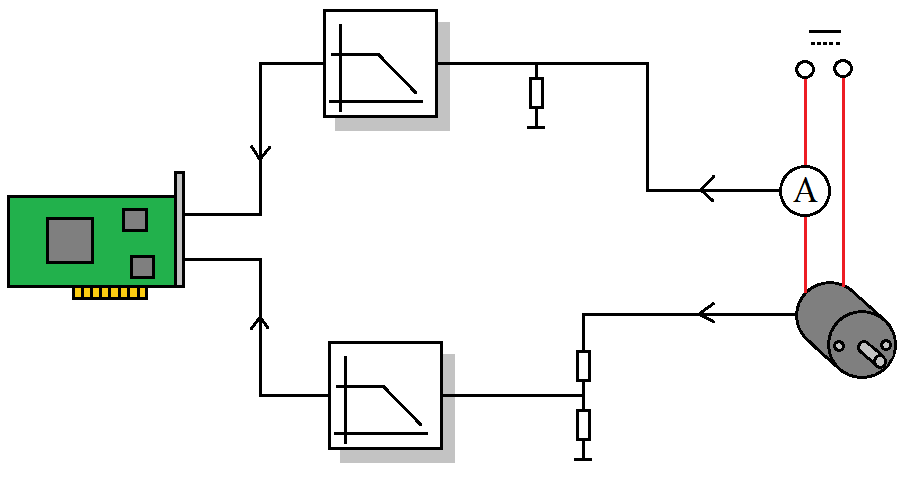
\includegraphics[width=1\textwidth]{Versuchasaufbau.png}
	\caption{Versuchsaufbau der Drehzahlmessung}
	\end{figure}

	
	Die Spannung, des Tachosignals ist zu groß, um sie direkt auf eine Messkarte zu geben. 
	Daher wird sie vorher mit einem Spannungsteiler im Verhältnis $1:10$
	herruntergeteilt. Um Allaising zu verhindern wird das Tachosignal anschließend mit 
	einem aktiven Filter gefiltert. Dann wird die Spannung mit der Messkarte erfasst.
	

	Der Strom wird mit einer Stromzange gemessen. Der Stromwandler gibt allerdings wieder 
	nur einen Strom aus. Dieser Strom wird mit einem Widerstand in eine Spannung umgewandelt. 
	Diese Spannung wird ebenfalls gefiltert und mit der 
	Messkarte aufgenommen. Der Filter wird einerseits genutzt, um den Gleichspannungsanteil 
	auszusperren und das Stromsignal zu verstärken, da sonst zu großes Quantisierungsrauschen entsteht.


\section{Einstellungen}

	Bevor der Versuch beginnt, sind die Abtastrate, die Messdauer und die
	Grenzfrequenzen der Antiallaisingfilter zu bestimmen. Die Messkarte besitzt eine maximale 
	Gesamtsamplerate von $200\frac{kS}{s}$. Diese Abtastrate kann auf die einzelnen
	Kanäle verteilt werden.


	Um eine möglichst hohe Auflösung zu erhalten, wird die maximale Abtastrate genutzt und auf 
	beide Kanäle gleichmäßig aufgeteilt. Jeder Kanal erhält also eine Samplerate
	von $100\frac{kS}{s}$. Um das Abtasttheorem einzuhalten, müssen alle Frequenzen
	über $50kHz$ zu null gedämpft werden. Daher wird die Grenzfrequenz der
	Antiallaisingfilter auf $40kHz$ eingestellt. Dieser wert wurde experimentell
	bestimmt. Für die Messdauer wurde nach einem Probelauf 15 Sekunden.
	gewählt.  
	

\section{Drehzahl bestimmen}

	Zunächst soll die Drehzahl des Motors durch das Tachosignal bestimmt werden. 
	Dazu werden die Funktionen aus den 
	Vorbereitungsaufgaben verwendet. Die Drehzahl wird einmal direkt im Zeitbereich 
	bestimmt und einmal durch eine Auswertung im Frequenzbereich.

	\begin{figure}[htb]
	\centering
	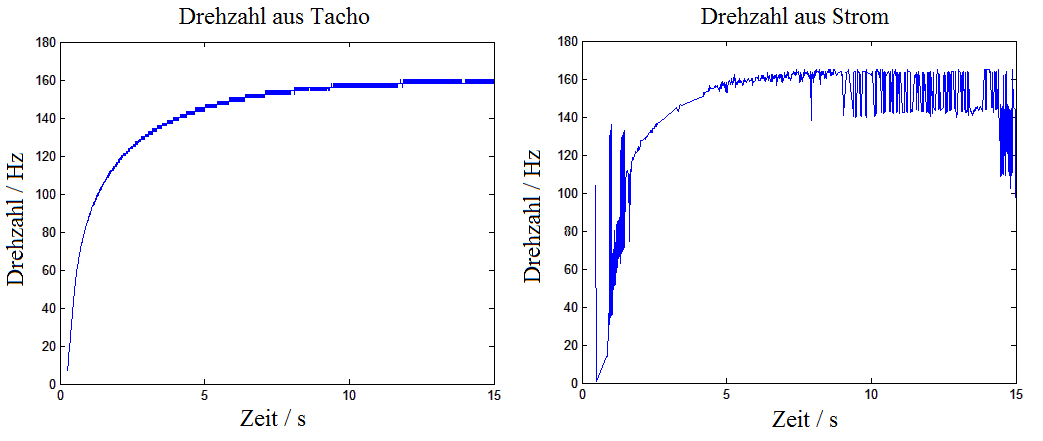
\includegraphics[width=1\textwidth]{zeitsignale.png}
	\caption{Drehzahl im Zeitbereich bestimmt}
	\end{figure}

	Die zeitliche Auflösung ist im Zeitbereich sehr gut. Da das Tachosignal nur eine Frequenz 
	zur Zeit enthält, kann diese auch noch gut bestimmt werden. Allerdings ist der
	Verlauf der Drehzahlkurve sprungartig. Die Frequenzauflösung ist also etwas grob. 
	Das Stromsignal enthält viele verschiedene Oberwellen. Die zeitliche Auflösung ist zwar immernoch 
	sehr gut, allerdings können die vielen verschiedenen Frequenzen nicht mehr richtig voneinander 
	getrennt werden. Pro Zeitpunkt ist nur eine Frequenz aus dem Plot ablesbar.
	Dennoch haben beide Kurven die selbe Tendenz. Das Tachosignal, liefert aber 
	wesendlich bessere Ergebnisse.

	\begin{figure}[htb]
	\centering
	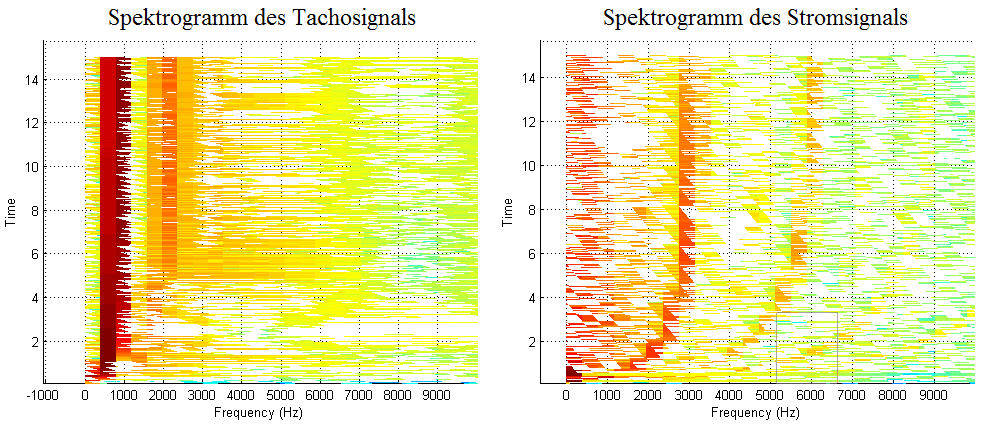
\includegraphics[width=1\textwidth]{frequenzsignale.png}
	\caption{Drehzahl im Zeitbereich bestimmt}
	\end{figure}

	Im Gegensatz zum Zeitbereich, sind im Frequenzbereich mehrere Frequenzen gleichzeitig zu erkennen. 
	Diese sind zeitlich aber nicht mehr so gut aufgelöst. Nun sind im Stromsignal meherer 
	Oberwellen zu erkennen. Die Verläufe der Oberwellen sind gut zu erkennen. Daher kann nun 
	einfach die Drehzahl bestimmt werden, wenn auch nur für 
	Zeitbereich und nicht für Zeitpunkte. Im Gegensatz dazu ist das Tachosignal wesendlich 
	schlechter zu erkennen. Es wurde zeitliche Auflösung aufgegeben um eine bessere Frequenzauflösung 
	zu erhalten. Diese ist aber wertlos, da eh nur eine Frequenz im Signal enthalten ist. 
	Zusätzlich kommt es durch die nicht unendliche Frequenzauflösung dazu, dass 
	die genaue Frequenz nicht genau erkannt werden kann. Das Spektrogramm des
	Tachosignals ist ungeeignet um die Drehzahl des Motors zu messen. Mit dem Spektrogramm des 
	Stroms sind hier wesendlich bessere Ergebnisse zu erzielen.


	Die zeitliche Messung des Tachosignals und die Frequenzmessung das Stroms ergeben eine 
	Drehzahl von ca. $9600\frac{U}{min}$. Die selbe Tendenz ist mit der
	zeitlichen Messung des Stroms zu erkennen, kann allerdings nicht so genau bestimmt werden. 
	Die Frequenzmessung des Tachosignals ist viel zu ungenau. Es wurde eine ungefähre Drehzahl von 
	$3750\frac{U}{min}$ erkannt, diese weicht aber zu stark von den anderen
	Messungen ab und sollte kritisch betrachtet werden.

\end{document}